
\chapter{CI for Exponentially Distributed (Censored) Data - Sundberg}

Let $X_1, \ldots , X_n$ be independent identically distributed random variables with rate $\theta \in (0, \infty)$.
In \cite{Sundberg2001} various methods for obtaining a confidence interval for $\theta$ given censored data are defined and tested.
\cite{Sundberg2001} mainly discusses CI based on type II censored data. In the following we will further obserbve the case of type I censored data and in the end discuss consequences for hybrid censored data.

\begin{table}[htbp]
	\centering
	\begin{tabular}{c|l|c|c|l}
		\hline
		Name & Used assumption & $c_l$ & $c_u$ & Notes \\
		\hline
		$C1$ & $\sqrt{n} \frac{\hat \theta - \theta}{\hat \theta} \sim \mathcal N (0, 1)$ & $1 - \frac{z_{1 - \frac{\alpha}{2}}}{\sqrt{n}}$ &  $1 + \frac{z_{1 - \frac{\alpha}{2}}}{\sqrt{n}}$ & \\
		$C2$ & $\sqrt{n} \frac{\hat \theta - \theta}{\theta} \sim \mathcal N (0, 1)$ &  $\frac{1}{1 + \frac{z_{1 - \frac{\alpha}{2}}}{\sqrt{n}}}$ &  $\frac{1}{1 - \frac{z_{1 - \frac{\alpha}{2}}}{\sqrt{n}}}$ & \\
		$C3$ & Delta method with $g(x) = \log(x)$ &  $\exp \left( - \frac{z_{1 - \frac{\alpha}{2}}}{\sqrt{n}} \right)$ &  $\exp \left( \frac{z_{1 - \frac{\alpha}{2}}}{\sqrt{n}} \right)$ & \\
		$C4$ & Delta method with $g(x) = x^{- \frac{1}{3}}$ & $\frac{1}{\left( 1 + \frac{z_{1 - \frac{\alpha}{2}}}{3 \sqrt{n}} \right)^3}$ & $\frac{1}{\left( 1 - \frac{z_{1 - \frac{\alpha}{2}}}{3 \sqrt{n}} \right)^3}$ & \\
		$C5$ & Likelihood function & & & $c_l$ and $c_u$ are the solutions of $2n \left( \frac{\hat \theta}{\theta} - 1 - \log \left( \frac{\hat \theta}{\theta}  \right) \right) \leq z_{1 - \frac{\alpha}{2}}^2$ \\
		$C6$ & & $\frac{2n}{\chi^2_{2n, 1 - \frac{\alpha}{2}}}$ &$\frac{2n}{\chi^2_{2n, \frac{\alpha}{2}}}$ & \\
		$C7$ & & $\frac{2n}{\chi^2_{2n+1, 1 - \frac{\alpha}{2}}}$ & $\frac{2n}{\chi^2_{2n+1, \frac{\alpha}{2}}}$ & \\
		\hline
	\end{tabular}
	\caption{Overview of the confidence intervals presented by \cite{Sundberg2001}.}
	\label{tab:confidence_intervals}
\end{table}

\textcolor{red}{($\star$) SUndberg CI methoden erst nach Zensierung einführen, dann zuerst ohne zensierung und dann mit zensierung}

\textcolor{red}{($\star$) This table should better be in the end of this section such that i can also include important information i discussed before, like when to use C7 instead of C6, ...}


First, calculate the MLE of the parameter $\theta$ and the Fisher information since we will need those values to construct a CI for $\theta$. For this we distinguish between the different censoring schemes. 

\paragraph{Uncensored:}

The likelihood function is given by
\[
L(\theta) = \prod_{i=1}^n \theta \exp(- \theta x_i)
= \theta^n \exp\!\Big(- \theta \sum_{i = 1}^n x_i\Big),
\]
and the log-likelihood function is
\begin{equation} \label{log likelihood function uncensored}
	\ell(\theta) = n \ln (\theta) - \theta \sum_{i = 1}^n x_i .
\end{equation}
Taking the first and second derivative with respect to $\theta$ gives
\[
\ell'(\theta) = \frac{n}{\theta} - \sum_{i = 1}^n x_i,
\qquad
\ell''(\theta) = - \frac{n}{\theta^2}.
\]

We obtain the MLE $\hat\theta$ by setting $\ell'(\theta) = 0$ and solving for $\theta$
\begin{equation} \label{MLE for uncensored}
	\frac{n}{\theta} - \sum_{i = 1}^n x_i = 0
	\quad \Longleftrightarrow \quad
	\hat\theta = \frac{n}{\sum_{i = 1}^n x_i}. 
\end{equation}
Since $\ell''(\theta) = -n/\theta^2 < 0$ for all $\theta > 0$, the log-likelihood function is strictly concave, so $\hat\theta$ is indeed the unique maximum.

The Fisher information is defined as the expected value of the negative second derivative of the log-likelihood function,
\[
\mathcal{I}(\theta) = \mathbb{E}\left[ - \ell''(\theta) \right].
\]
In this case, $-\ell''(\theta) = n/\theta^2$ does not depend on the data $x_1, \ldots, x_n$. 
Hence it is not random, and its expected value is the constant itself
\begin{equation} \label{fisher info exp uncensored}
	\mathcal{I}(\theta)
	=
	\mathbb{E} \left[ \frac{n}{\theta^2} \right]
	=
	\frac{n}{\theta^2}.
\end{equation}

We will use $\hat\theta$ and $\mathcal{I}(\theta)$ later to construct confidence intervals.

\paragraph{Type-II censored data}
Surprisingly, type-II censored data leads to results that are similar to those for uncensored data.
Let $r \in \{1, \ldots, n\}$ be fixed and let $Y_1, \ldots, Y_n$ be the type-II censored data corresponding to $X_1, \ldots, X_n$.

The likelihood function is
\begin{align*}
	L(\theta) 
	&=
	\underbrace{\prod_{i=1}^r \theta \exp(- \theta x_{i:n})}_{\text{uncensored}} \cdot \underbrace{\exp(- \theta x_{r:n})^{n-r}}_{\text{censored}} \\
	&=
	\theta^r \exp \Bigg( - \theta \bigg[ \underbrace{\sum_{i = 1}^r x_{i:n} + (n-r)\, x_{r:n}}_{=:S} \bigg] \Bigg),
\end{align*}
and the log-likelihood function and its derivatives are
\begin{align}
	\ell(\theta) &= r \ln \theta - \theta S, \label{log likelihood function type II censored} \\
	\ell'(\theta) &= \frac{r}{\theta} - S, \notag \\
	\ell''(\theta) &= - \frac{r}{\theta^2}. \notag
\end{align}
Setting $\ell'(\theta) = 0$ gives the MLE
\begin{equation}  \label{MLE for type II censored}
	\hat\theta = \frac{r}{S}.
\end{equation}
Again, the second derivative does not depend on the data, so the Fisher information is
\begin{equation} \label{fisher info exp type II}
	\mathcal{I}(\theta) = \mathbb{E}\left[ - \ell''(\theta) \right] = \frac{r}{\theta^2}.
\end{equation}

These are the same formulas as in the uncensored case with the change that
the sample size $n$ is replaced by the number $r$ of observed failures, and the sum of the observations $\sum_{i=1}^n x_i$ is replaced by the sum of the censored observations
\[
S = \sum_{i = 1}^n y_i = \sum_{i = 1}^r x_{i:n} + (n-r)\, x_{r:n}.
\]
For $r = n$ we have $S = \sum_{i=1}^n x_i$, so the uncensored case is included as a special case.


\paragraph{Type-I censored data}

Let $c > 0$ be a fixed time at which the experiment is stopped, and let $Y_1, \ldots, Y_n$ be the corresponding type-I censored data, i.e.\ $Y_i = \min(X_i, c)$.
Again, we start by computing the likelihood function
\begin{align*}
	L(\theta) 
	&=
	\underbrace{\prod_{i=1}^R \theta \exp(- \theta x_{i:n})}_{\text{uncensored}} \cdot \underbrace{\exp(- \theta c)^{n-R}}_{\text{censored}} \\
	&=
	\theta^R \exp \Bigg( - \theta \bigg[ \underbrace{\sum_{i = 1}^R x_{i:n} + (n-R)\,c}_{=:S} \bigg] \Bigg),
\end{align*}
where $R$ is the number of uncensored observations, i.e.\ the number of $X_i$ with $X_i \leq c$.
In contrast to type-II censoring, $R$ is not fixed but a random variable.
Each observation $X_i$ is uncensored with probability
\[
p = \mathbb{P}(X_i \leq c) = 1 - \exp(-\theta c),
\]
and the observations are independent. 
Hence $R$ is binomially distributed
\[
R \sim \text{Bin}\big(n,\, 1 - \exp(-\theta c)\big).
\]

The log-likelihood function and its derivatives are given by
\begin{align*}
	\ell(\theta) &= R \ln \theta - \theta S, \\
	\ell'(\theta) &= \frac{R}{\theta} - S, \\
	\ell''(\theta) &= - \frac{R}{\theta^2}.
\end{align*}
For $R \geq 1$, setting $\ell'(\theta) = 0$ gives the MLE
\[
\hat\theta = \frac{R}{S},
\]
where $S$ depends on the data and on the random variable $R$.
For $R = 0$ we have $\ell'(\theta) = -S = -nc < 0$ for all $\theta$, so $\ell$ is strictly decreasing and the MLE does not exist.

This time, the Fisher information is not a constant, because the random variable $R$ appears in the second derivative
\[
\mathcal{I}(\theta) 
= 
\mathbb{E} \left[ - \ell''(\theta) \right]
=
\mathbb{E} \left[ \frac{R}{\theta^2} \right]
=
\frac{\mathbb{E}[R]}{\theta^2} 
=
\frac{n \left( 1 - \exp(-c \theta) \right)}{\theta^2}.
\]

Compared to the uncensored case, the Fisher information has the extra factor $1 - \exp(-c\theta)$.
This is exactly the probability that an observation is uncensored.
Equivalently, the sample size $n$ is replaced by the expected number of observed failures $\mathbb{E}[R]$, as $r$ replaced $n$ in the type-II case.
The factor shows how much information is lost by censoring.
\begin{itemize}
	\item For $c \to \infty$, we have $1 - \exp(-c\theta) \to 1$ and we recover the information $n/\theta^2$ of the uncensored case.
	\item For $c \to 0$, we have $1 - \exp(-c\theta) \to 0$, so almost all observations are censored and the data contain almost no information about $\theta$.
\end{itemize}


\section{C1}

By the asymptotic normality of the MLE $\hat\theta$, it holds that
\begin{equation} \label{fisher info exp}
	\sqrt{\mathcal{I}(\theta)} \left( \hat\theta - \theta \right) 
	\overset{d}{\longrightarrow}
	\mathcal{N}(0, 1).
\end{equation}
The MLE is consistent, i.e.\ $\hat\theta \overset{P}{\longrightarrow} \theta$ \textcolor{red}{($\star$)}.
The mapping $g(t) = \theta / t$ is continuous on $(0, \infty)$ and with the continuous mapping theorem holds
\begin{equation}
	\hat\theta \overset{P}{\longrightarrow} \theta 
	\overset{CMT}{\implies }
	g(\hat\theta) \overset{P}{\longrightarrow} g(\theta)
	\implies
	\frac{\theta}{\hat \theta} 
	\overset{P}{\longrightarrow} \frac{\theta}{ \theta} = 1.
\end{equation}
We can describe the Fisher information of the uncensored and the type-II censored case derived in \eqref{fisher info exp uncensored} and \eqref{fisher info exp type II} as $\mathcal I (\theta) = m / \theta^2$ with $m \in \{n, r\}$.
We can conclude that 
\begin{equation}
	\sqrt{\frac{\mathcal I (\hat \theta)}{\mathcal I (\theta)} }
	=
	\sqrt{\frac{m / \hat \theta^2}{m / \theta^2}}
	=
	\frac{\theta}{\hat \theta} 
	\overset{P}{\longrightarrow}
	1.
\end{equation}
This holds for the Fisher information of the uncensored and the type-II censored case.
Together with~\eqref{fisher info exp}, Slutsky's theorem gives
\begin{equation} \label{distn for C1}
	\sqrt{\mathcal{I}(\hat\theta)} \left( \hat\theta - \theta \right)
	=
	\sqrt{\frac{\mathcal{I}(\hat\theta)}{\mathcal{I}(\theta)}}
	\cdot
	\sqrt{\mathcal{I}(\theta)} \left( \hat\theta - \theta \right)
	\overset{d}{\longrightarrow}
	1 \cdot \mathcal{N}(0, 1).
\end{equation}

With the knowledge of the asymptotic distribution of the standardized MLE in~\eqref{distn for C1}, one can construct an approximate confidence interval.
Let $z_p$ denote the $p$-quantile of the standard normal distribution. We directly utilize the fact that $z_{\alpha/2} = -z_{1-\alpha/2}$. 
For large $m$ it holds that
\begin{align*}
	1 - \alpha 
	&\approx
	\mathbb{P} \left( z_{\alpha / 2} \leq \sqrt{\mathcal{I}(\hat\theta)} \left( \hat\theta - \theta \right) 
	\leq z_{1 - \alpha / 2} \right) \\
	&=
	\mathbb{P} \left( -z_{1 - \alpha / 2} \leq \sqrt{m}\, \frac{\hat\theta - \theta}{\hat\theta}  
	\leq z_{1 - \alpha / 2} \right)
\intertext{and rearranging for $\theta$ gives}
	&=
	\mathbb{P} \left( \hat\theta \left( 1 - \frac{z_{1 - \alpha / 2}}{\sqrt{m}} \right) \leq \theta \leq \hat\theta \left( 1 + \frac{z_{1 - \alpha / 2}}{\sqrt{m}} \right) \right).
\end{align*}
Hence an approximate $(1 - \alpha)$-confidence interval for $\theta$ is given by
\begin{equation*}
	C1_{1 - \alpha} = \left[\, \hat\theta \left( 1 - \frac{z_{1 - \alpha / 2}}{\sqrt{m}} \right),\; \hat\theta \left( 1 + \frac{z_{1 - \alpha / 2}}{\sqrt{m}} \right) \right].
\end{equation*}


\section{C2}

We can also directly use the resulting distribution from the asymptotic normality of the MLE presented in~\eqref{fisher info exp} and use it to derive a CI.

\begin{align*}
	1 - \alpha
	&\approx
	\mathbb{P} \left( z_{\alpha / 2} \leq \sqrt{\mathcal{I}(\theta)} \left( \hat\theta - \theta \right) 
	\leq z_{1 - \alpha / 2} \right) \\
	&=
	\mathbb{P} \left( -z_{1 - \alpha / 2} \leq \sqrt{m}\, \frac{\hat\theta - \theta}{\theta}  
	\leq z_{1 - \alpha / 2} \right)
\intertext{and rearranging gives} 
	&=
	\mathbb{P} \left( 
	\frac{\hat \theta}{1 - \frac{z_{1 + \alpha / 2}}{\sqrt{m}}}
	\leq 
	\theta
	\leq 
	\frac{\hat \theta}{1 + \frac{z_{1 - \alpha / 2}}{\sqrt{m}}}
	\right).
\end{align*}
So an approximate $(1-\alpha)$-CI  is given by
\begin{equation*}
	C2_{1 - \alpha} = \left[
	\frac{\hat \theta}{1 + \frac{z_{1 - \alpha / 2}}{\sqrt{m}}}, 
	\frac{\hat \theta}{1 - \frac{z_{1 - \alpha / 2}}{\sqrt{m}}}
	\right].
\end{equation*}

\textcolor{red}{($\star$) Was unterscheidet C2 von C1, was ist besser}

\textcolor{red}{($\star$) Problem mit $N \in \{1, 2\}$ erklären}

For certain small sample sizes $n$, the interval $C2_{1-\alpha}(\theta)$ has a negative upper bound and a positive lower bound. In this case, it is not a valid interval. This can be seen in Figure~\ref{fig:sundberg_alpha_comparison}, which plots the sample size $n$ against the quantity $c_u - c_l$. This quantity is proportional to the width of the interval. The exact width is obtained by multiplying $c_u - c_l$ by $\hat\theta_n$.

The range of small $n$ for which $c_u - c_l$ is negative depends on $\alpha$. 
For $\alpha = 0.01$, the interval is invalid for $n \leq 6$, as shown in Figure~\ref{fig:sundberg_alpha_001}.
For $\alpha = 0.1$, the interval is invalid for $n \in \{0, 1, 2\}$, as shown in Figure~\ref{fig:sundberg_alpha_01}. 

It holds 
\[
\frac{z_{1- \frac{\alpha}{2}}}{\sqrt{n}} > 1
\quad \text{if and only if} \quad
n < z_{1-\alpha/2}^2
\]
and exactly in this case, the denominator of the upper bound $1 - \frac {z_{1-\alpha/2}}{\sqrt{n}}$ is negative, while the lower bound is always positive for all $n \in \mathbb N _0$ and $\alpha \in (0, 1)$. 
So the confidence interval $C2_{1-\alpha}(\theta)$ is invalid if $n < z_{1 - \frac{\alpha}{2}}^2$.

The range of $n$ changes with $\alpha$ because the critical value $z_{1-\alpha/2}^2$ increases as $\alpha$ decreases. In other words, a smaller significance level leads to a larger critical value, which increases the range of sample sizes for which $c_u$ is negative.

For example, when $\alpha = 0.1$, the interval is invalid for all
\[
n < z_{0.95}^2 \approx 2.706.
\]
When $\alpha = 0.01$, the interval is invalid for all
\[
n < z_{0.995}^2 \approx 6.635.
\]
Thus, a smaller significance level results in a larger range of sample sizes for which the interval is invalid. This is consistent with the observations shown in Figure~\ref{fig:sundberg_alpha_comparison}.

\begin{figure}[htbp]
	\centering
	
	\begin{subfigure}[b]{0.48\textwidth}
		\centering
		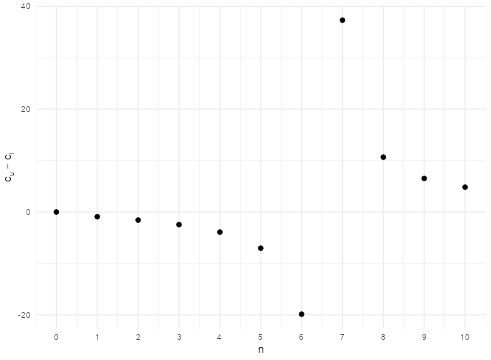
\includegraphics[width=\textwidth]{figures/sundberg_C2/C2_Sundberg_alpha_0.01.png}
		\caption{$\alpha = 0.01$}
		\label{fig:sundberg_alpha_001}
	\end{subfigure}
	\hfill
	\begin{subfigure}[b]{0.48\textwidth}
		\centering
		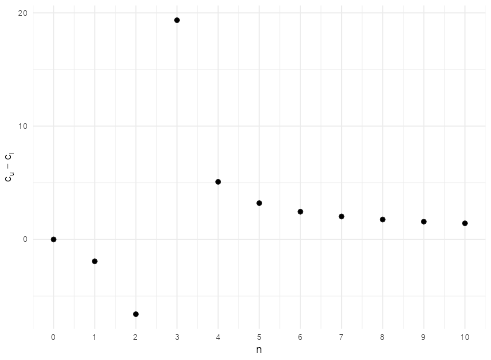
\includegraphics[width=\textwidth]{figures/sundberg_C2/C2_Sundberg_alpha_0.1.png}
		\caption{$\alpha = 0.1$}
		\label{fig:sundberg_alpha_01}
	\end{subfigure}
	
	\caption{Quantity $c_u - c_l$ for the multiplier of confidence interval $C2_{1-\alpha} (\theta)$ for different $\alpha$}
	\label{fig:sundberg_alpha_comparison}
\end{figure}

\section{C3}


\cite{Sundberg2001} uses the delta method to obtain a standard normal limit distribution, on which he bases the confidence interval C3 \textcolor{red}{($\star$) C3, C4: which CIs are meant?}.

For this method, we first rearrange~\eqref{fisher info exp} to obtain
\begin{equation*}
	\sqrt{\mathcal{I}(\theta)} \left( \hat\theta - \theta \right) 
	=
	\sqrt{m} \Big( \underbrace{\frac{\hat\theta}{\theta}}_{=:\, Z_m} - 1 \Big).
\end{equation*}
and by~\eqref{fisher info exp} the right side also converges in distribution, i.e.\ $\sqrt{m} \left( Z_m - 1 \right) \overset{d}{\longrightarrow} \mathcal{N}(0, 1)$.

We now apply the delta method with the function $g(x) = \log x$.
It holds that $g'(1) = 1 \neq 0$, so the conditions of the delta method are satisfied, and we obtain
\begin{equation*}
	\sqrt{m} \left( g(Z_m) - g(1) \right) \overset{d}{\longrightarrow} \mathcal{N} \left( 0, \, |g'(1)|^2 \right).
\end{equation*}
Since $g(Z_m) - g(1) = \log(\hat\theta / \theta) - \log 1 = \log \hat\theta - \log \theta$ and $|g'(1)|^2 = 1$, this simplifies to
\begin{equation*}
	\sqrt{m} \left( \log \hat\theta - \log \theta \right) \overset{d}{\longrightarrow} \mathcal{N}(0, 1).
\end{equation*}
This is the distribution used to construct C3 in~\cite{Sundberg2001}. For sufficiently large $m$ holds
\begin{align*}
	1 - \alpha 
	\approx&
	\mathbb{P} \left( z_{\alpha / 2} \leq \sqrt{m} \left( \log \hat\theta - \log \theta \right) \leq z_{1 - \alpha / 2} \right)
\intertext{and rearranging gives}
	=&
	\mathbb{P} 
	\left( 
	\hat \theta  \cdot \exp \left( - \frac{z_{1 - \alpha / 2}}{\sqrt{m}} \right)
	\leq \theta \leq 
	\hat \theta \cdot \exp \left( \frac{z_{1 - \alpha / 2}}{\sqrt{m}} \right)
	\right).
\end{align*}
So another $(1 - \alpha)$-CI is given by 
\begin{equation*}
	C3_{1 - \alpha} = 
	\left[
	\hat \theta  \cdot \exp \left( - \frac{z_{1 - \alpha / 2}}{\sqrt{m}} \right)
	,
	\hat \theta \cdot \exp \left( \frac{z_{1 - \alpha / 2}}{\sqrt{m}} \right)
	\right].
\end{equation*}

\textcolor{red}{($\star$) What about type I censoring?}

\section{C4}


Again, we will use the delta method but this time with~\eqref{distn for C1} and the mapping $g(x) = x^{-1/3}$. We will similiarily to the method of C3 first observe that
\begin{align}
	\sqrt{\mathcal I (\hat \theta)} \left( \hat \theta - \theta \right) = 
	\sqrt{m} \Bigg( 1 - g\bigg( \underbrace{\frac{\theta}{\hat \theta}}_{=: Z_m} \bigg) \Bigg)
\end{align}
is normally distributed as we saw in~\eqref{distn for C1}. 
It holds $g(Z_m) =\left(  \frac{\hat \theta}{\theta} \right)^{\frac{1}{3}}, g(1) = 1$ and $|g'(1)|^2 = \frac{1}{9}$. So 
\begin{align*}
	\sqrt{m} \left( g(1) - g(Z_m) \right) \overset{d}{\rightarrow} \mathcal N \left( 0, \frac{1}{9} \right)
\intertext{what simplfies to}
	\sqrt{m} \left( \frac{\theta^{1 / 3} - \hat \theta^{1 / 3}}{\theta^{1 / 3}} \right) \overset{d}{\rightarrow} \mathcal N \left( 0, \frac{1}{9} \right).
\end{align*}
To get the standard normal distribution, one can multiply by $3$ what gives us
\begin{align}
	3 \sqrt{m} \left( \frac{\theta^{1 / 3} - \hat \theta^{1 / 3}}{\theta^{1 / 3}} \right) \overset{d}{\rightarrow} \mathcal N \left( 0, 1 \right). \label{distn for C4}
\end{align}

Using \eqref{distn for C4} gives for large $m$
\begin{align}
	1 - \alpha 
	&\approx
	\mathbb{P} 
	\left( 
		z_{\alpha / 2} 
		\leq
		3 \sqrt{m} \left( \frac{\theta^{1 / 3} - \hat \theta^{1 / 3}}{\theta^{1 / 3}} \right)
		\leq
		z_{1 - \alpha / 2}
	\right)
\intertext{what can be rearranged to}
	&=
	\mathbb{P} 
	\left( 
	\frac{\hat \theta}{\left( 1 + \frac{z_{1 - \alpha / 2}}{3\sqrt{m}} \right)^3}
	\leq
	\theta
	\leq
	\frac{\hat \theta}{\left( 1 - \frac{z_{1 - \alpha / 2}}{3\sqrt{m}} \right)^3}
	\right)
\end{align}
All in all, we get the approximate CI
\[
C4_{1-\alpha}
=
\left[
\frac{\hat \theta}{\left( 1 + \frac{z_{1 - \alpha / 2}}{3 \sqrt{m}} \right)^3} 
,
\frac{\hat \theta}{\left( 1 - \frac{z_{1 - \alpha / 2}}{3 \sqrt{m}} \right)^3}
\right].
\]

\textcolor{red}{($\star$) what about type I censoring?}

\section{C5}




Likelihood-based CI

Wilks Theorem:
\[
2 \left\{ l(\hat \theta) - l(\theta) \right\}
\overset{d}{\longrightarrow} 
\chi_1^2
\]



For uncensored and type-II censored data, the log likelihood function is given by~\eqref{log likelihood function uncensored} and~\eqref{log likelihood function type II censored}. We can again generalize this with $m \in \{n , r\}$ is the log likelihood given by 
\begin{equation*}
	\ell (\theta) = m \log (\theta) - \theta S
\end{equation*}
with 
\[
	S = \sum_{i = 1}^n y_i = \sum_{i = 1}^r x_{i:n} + (n-r) x_{r:n}.
\]
With basic calculus and substituting the MLE $\hat \theta = m / S$ from~\eqref{MLE for uncensored} and \eqref{MLE for type II censored} follows
\begin{align} \label{log likelihood wilk}
	2 \left( \ell(\hat \theta) - \ell (\theta) \right) 
	=
	2 m \left( \frac{\theta}{\hat \theta}  - 1 - \log \left( \frac{\theta}{\hat \theta} \right)\right).
\end{align}

Wilks Theorem delivers, that~\eqref{log likelihood wilk} is $\chi_1^2$ in distribution, so for large $m$ holds
\begin{align*}
	1 - \alpha \approx
	\mathbb{P} 
	\left( 
		2 m \left( \frac{\theta}{\hat \theta}  - 1 - \log \left( \frac{\theta}{\hat \theta} \right)\right) 
		\leq 
		\chi^2_{1, 1 - \alpha}
	\right)
\end{align*}
where we denote the $p$ quantile fo the $\chi^2_1$ distribution as $\chi^2_{1, p}$. Also we can use the key identity $\chi^2_{1, 1 - \alpha} = z_{1 - \alpha / 2}^2$ \textcolor{red}{($\star$) find source} and obtain the $C5_{1- \alpha}$ by using the solutions of the inequality
\[
	2 m \left( \frac{\theta}{\hat \theta}  - 1 - \log \left( \frac{\theta}{\hat \theta} \right)\right) 
	\leq 
	z_{1 - \alpha / 2}^2
\]
as bounds of the CI.

\section{C6}


The total sum of observations $S$ can be expressed in terms of the normalized spacings \textcolor{red}{($\star$) spacings besser erklären, wurden diese schonmal erwähnt?}
\[
	D_i := (n-i+1) \left( X_{i:n} - X_{(i-1):n} \right)
\]
for $i \in \{1, \ldots , r\}$ which are iid $\text{Exp}(\theta)$ distributed and 
\[
	S = \sum_{i = 1}^r D_i.
\] 
The sum of independent exponentially distributed random variables is Gamma distributed i. e. 
\[
	S \sim \text{Gamma}(r, \theta)
\]
and normalizing this gives
\[
	2 \theta S \sim \text{Gamma} \left( r, \frac{1}{2} \right) = \chi^2_{2r}
\]

\begin{align*}
	1 - \alpha 
	=& 
	\mathbb{P} \left( \chi^2_{2r, \alpha / 2} 
	\leq 
	2 \theta S
	\leq 
	\chi^2_{2r, 1 - \alpha / 2}
	\right) \\
	=&
	\mathbb{P} \left( \frac{\chi^2_{2r, \alpha / 2}}{2S} 
	\leq 
	\theta
	\leq 
	\frac{\chi^2_{2r, 1 - \alpha / 2}}{2S}
	\right) \\
\intertext{and using the MLE $\hat \theta = m / S$ gives}
	=&
	\mathbb{P} \left( 
	\frac{\chi^2_{2r, \alpha / 2}}{2r} \hat \theta 
	\leq 
	\theta
	\leq 
	\frac{\chi^2_{2r, 1 - \alpha / 2}}{2r} \hat \theta
	\right)
\end{align*}

so an exact $(1- \alpha)$ CI for $\theta$ is given by 
\[
	C6_{1 - \alpha} = \left[ 
	\frac{\chi^2_{2r, \alpha / 2}}{2r} \hat \theta 
	,
	\frac{\chi^2_{2r, 1 - \alpha / 2}}{2r} \hat \theta
	\right]
\]

\textcolor{red}{($\star$) what about type I?}

\section{C7}

\[
C7_{1 - \alpha} = \left[ 
\frac{\chi^2_{2r+1, \alpha / 2}}{2r} \hat \theta 
,
\frac{\chi^2_{2r+1, 1 - \alpha / 2}}{2r} \hat \theta
\right]
\]


\textcolor{red}{($\star$) Wieso kann ich diese heuristik anwenden?}





\textcolor{red}{($\star$) Auch an anderen beispielen austesten}

\textcolor{red}{($\star$) Ich möchte generell in allen Ci von Sundberg die herleitung kleinschrittiger machen sodass bezüglich dieser Intervalle keine Fragen mehr offen bleiben (genau die zugrundeliegende verteilung erklären und warum diese gilt, die Umformung zum standardized und zum CI vornehmen)}

\textcolor{red}{($\star$) am ende oder anfang tabelle mit allen CI und deren zugrundeliegenden Annahmen erstellen (das auch für die CI von Jeng zB)}

\section{Figures aus Sundberg replizieren}
Non-Coverage probabilities simulieren



